%% LaTeX-Beamer template for KIT design
%% by Erik Burger, Christian Hammer
%% title picture by Klaus Krogmann
%%
%% version 2.1
%%
%% mostly compatible to KIT corporate design v2.0
%% http://intranet.kit.edu/gestaltungsrichtlinien.php
%%
%% Problems, bugs and comments to
%% burger@kit.edu

\documentclass[18pt]{beamer}
\usepackage[utf8]{inputenc}
%% SLIDE FORMAT

% use 'beamerthemekit' for standard 4:3 ratio
% for widescreen slides (16:9), use 'beamerthemekitwide'

\usepackage{templates/beamerthemekit}
% \usepackage{templates/beamerthemekitwide}

%% TITLE PICTURE

% if a custom picture is to be used on the title page, copy it into the 'logos'
% directory, in the line below, replace 'mypicture' with the 
% filename (without extension) and uncomment the following line
% (picture proportions: 63 : 20 for standard, 169 : 40 for wide
% *.eps format if you use latex+dvips+ps2pdf, 
% *.jpg/*.png/*.pdf if you use pdflatex)

%\titleimage{mypicture}

%% TITLE LOGO

% for a custom logo on the front page, copy your file into the 'logos'
% directory, insert the filename in the line below and uncomment it

%\titlelogo{mylogo}

% (*.eps format if you use latex+dvips+ps2pdf,
% *.jpg/*.png/*.pdf if you use pdflatex)

%% TikZ INTEGRATION

% use these packages for PCM symbols and UML classes
% \usepackage{templates/tikzkit}
% \usepackage{templates/tikzuml}

% the presentation starts here

\title[Geometrie 2]{Geometrie 2 - ICPC Praktikum SS14}


\institute{Tobias Hornberger $\cdot$ Paul Jungeblut $\cdot$ Enja Stein $\cdot$ Lena Winter}

\begin{document}

% change the following line to "ngerman" for German style date and logos
\selectlanguage{ngerman}

%title page
\begin{frame}
\titlepage
\end{frame}

\section{Konvexe Hülle}
	\subsection{Problemstellung}
		\begin{frame}{Problemstellung: Konvexe Hülle}
			\begin{box}
			 Gegeben sei eine Menge M von Punkten in der Ebene. Die konvexe Hülle von M ist die kleinste konvexe Menge, in der M enthalten ist.
			\end{box}
			\begin{figure}
				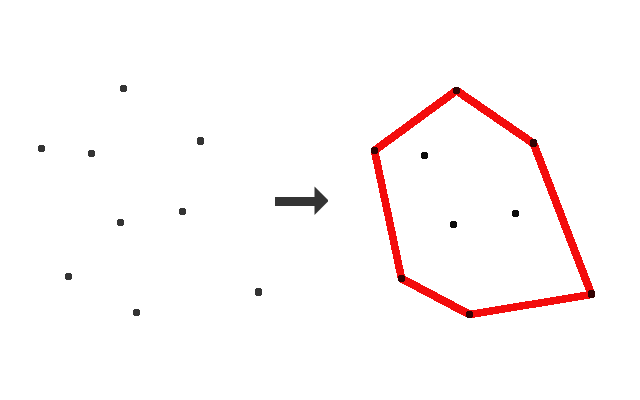
\includegraphics[width=8cm]{logos/konhu.png}\\
			\end{figure}
		\end{frame}
	
	\subsection{Graham Scan}
		\begin{frame}{Idee: Graham Scan}
	
		\end{frame}
	
		\begin{frame}{Pseudocode}
	
		\end{frame}

\section{Sweepline}

	\subsection{Problemstellung}
		\begin{frame}{Problemstellung: Linienschnitt}
		\end{frame}
	
	\subsection{Sweepline}
		\begin{frame}{Idee: Sweepline}
	
		\end{frame}
	
		\begin{frame}{Pseudocode}
	
		\end{frame}
	
\section{Closed Pair}

	\subsection{Problemstellung}
		\begin{frame}{Problemstellung: Closed Pair}
			\textbf{Geben:} n Punkte auf einer Ebene \\
			\textbf{Gesucht:} die beiden am nähesten zusammenliegenden Punkte\\
		
			\begin{block}{Naiver Ansatz}
				Mit Vollständiger Suche. \\
				\ \\
				Alle Distanzen zwischen allen möglichen Punktpaaren ausrechnen und davon das Minimum wählen. 
				\ \\
				\textbf{Laufzeit:} $\mathcal{O}(n^2)$
			\end{block}	
		\end{frame}
	
	\subsection{Divide and Conquer}
		\begin{frame}{Idee: Divide and Conquer}
			Statt Vollständiger Suche: Divide \& Conquer für eine Lösung in $\mathcal{O}(n \log n)$ Zeit.

			\begin{enumerate}
				\item \textbf{Divide}:\\ Sortieren der Punkte (Primär x-Koordinate, sekundär y-Koordinate). Aufteilen der Punktmenge in zwei Hälften
				\item \textbf{Conquer}:\\ Größe der Punktmengen:
					\begin{itemize}
						\item $|$Punktmenge$|$ = 1, return $ \infty$
						\item $|$PunktMenge$|$ = 2, return Euklidische Distanz der beiden Punkte
					\end{itemize}
				\item \textbf{Combine}: \\ Sei $d_{1}$ die kleinste Distanz innerhalb der Punktmenge $A_1$. \\
							Sei $d_2$ die kleinste Distanz innerhalb der Punktmenge $A_2$. \\
							Sei $d_{3}$ die kleinste Distanz von 2 Punkte aus jeweils $A_{1}$ und $A_{2}$.\\
							$\rightarrow$ Die kleinste Distanz innerhalb $A_1$ $\cup$ $A_2$ ist $\min(s_1,s_2, s_3)$ \\
			\end{enumerate}
		\end{frame}

		\begin{frame}{Combine}
			Naiver Ansatz für Combine immer noch in Laufzeit $\mathcal{O}(n^2)$ \\
			\centerline{\huge{Optimierbar!}} \\
			Sei $d' = \min(d_1, d_2)$. \\  
			Für jeden Punkt in der unteren Punktmenge kann der nähere Punkt nur in einem Rechteck mit Breite $d' \text{und Höhe} 2*d'$ liegen
			\begin{block}{Beweisbar}
				Es gibt maximal 6 solche Punkte im Rechteck. \\
				Ohne Beweis
			\end{block}
			\ \\
			$\Rightarrow$ Maximal $\mathcal{O}(6n)$ Operationen für Combine \\
			$\Rightarrow$ \textbf{Gesamtlaufzeit:} \\ $T(n) = 2 * T(n/2) + \mathcal{O}(n)$, und es gilt: $T(n) \in \mathcal{O}(n \log n)$
		\end{frame}
	
		\begin{frame}{Pseudocode}
	
		\end{frame}
	

\end{document}
